%\documentclass[a4paper,english,11pt,twoside]{article}
\documentclass[a4paper,english,11pt]{article}

\usepackage[utf8]{inputenc}
\usepackage[T1]{fontenc, url}
\usepackage[english]{babel}
%\usepackage{epsfig}
\usepackage{graphicx}
\usepackage{amsmath}
\usepackage{mathtools}
\usepackage{pstricks}
\usepackage{subfig}
\usepackage{epstopdf}
\usepackage{varioref}
\usepackage{listings}
\usepackage{xcolor}
\usepackage{float}
\usepackage[]{mcode}
\usepackage{verbatim}
\lstset{ 
  captionpos=b,
  frame=tb,
  numbers=left}
\urlstyle{sf}
\usepackage[margin=1 in]{geometry} % Setter margene til word standard

\usepackage{ifikompendiumforside}


\newcommand{\tab}[1]{\hspace{.2\textwidth}\rlap{#1}}

\newcommand{\itab}[1]{\hspace{0em}\rlap{#1}}

%%%%%%%%%%%%%%%%%% END HEADER

\title{Laboratory Assignment 2}
\subtitle{INF4411\\ 
          Analog Microelectronics}

\author{
\begin{tabular}{ r c l }
  Rikesh Chauhan & & rikesh.chauhan@fys.uio.no\\
  Espen Klein Nilsen & & e.a.k.nilsen@fys.uio.no\\
  Vegard Midtbøen & & vegard.midtboen@fys.uio.no
\end{tabular}
}
%{Rikesh Chauhan rikesh.chauhan@fys.uio.no\\
%	Espen Klein Nilsen e.a.k.nilsen@fys.uio.no\\
%	Vegard Midtbøen vegard.midtboen@fys.uio.no} 

\begin{document}
\ififorside

\tableofcontents

\newpage
%//////////////////////////////////////Task1///////////////////////////////////////////////////////////////////////        
\section{Task 1}
The first task was to find a proper bias voltage in order to get a pMOS transitor to deliver a current of $20 {\mu} A$.
The transistor that was used is a MC14007UBCP.
We chose $V_{DD}$ i.e. $V_s$ to be $5 V$ and $V_d$ to be $2.5 V$, which results Vsd to be $2.5 V$. We choose this so that the $20 {\mu} A$ point
lies around the middle when sweeing $V_{sweep} = 0-5V$ and hence we can see the plot before and after this point.\\ 
\\
The circut is shown in Figure \ref{fig:sch:task1}.\\
\begin{figure}[!htbp]
 \centering
  \fbox{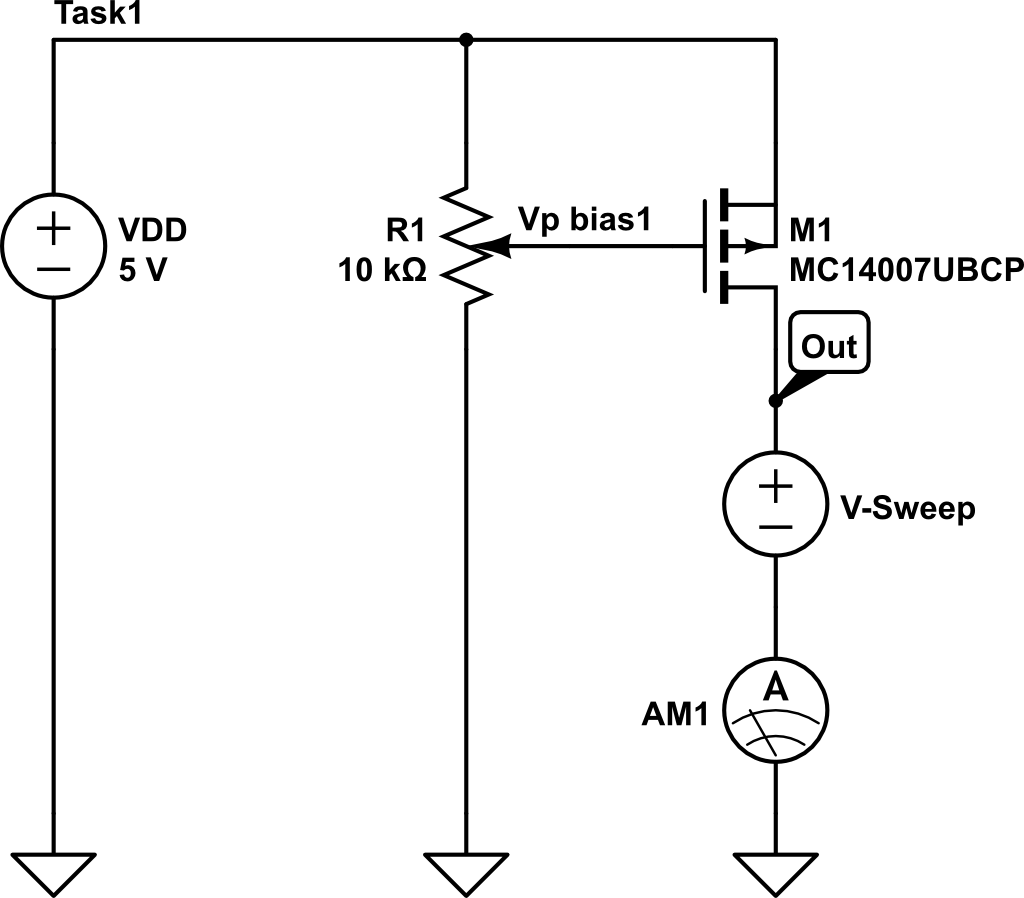
\includegraphics[width=0.5\textwidth]{img/inf4411_lab2_task1_schematics.png}}
  \caption{Shematic for one pMOS transistor.}
  \label{fig:sch:task1}	
\end{figure}
\\
In order to get a proper bias voltage ($V_{p\_bias1}$), 
we used a potentiometer of $10k\Omega$ which is used as a voltage divider in order to bias pMOS. 
This bias voltage was found to be $1.196 V$ realtive to $V_{DD}$ in order to match the given drain current.\\
Similarly output resistance $r_{ds} = 391k\varOmega$.
The result of the experiment is shown in the Figure \ref{fig:pmos-as-current-source}.\\
\\
The minimal $V_{out}$ for this circuit to act as an current source is $V_{DD} - V_{sd} = V_{out}$, $5 V - 0.5 V = 4.5 V$
\begin{figure}[!htbp]
 \centering
  \fbox{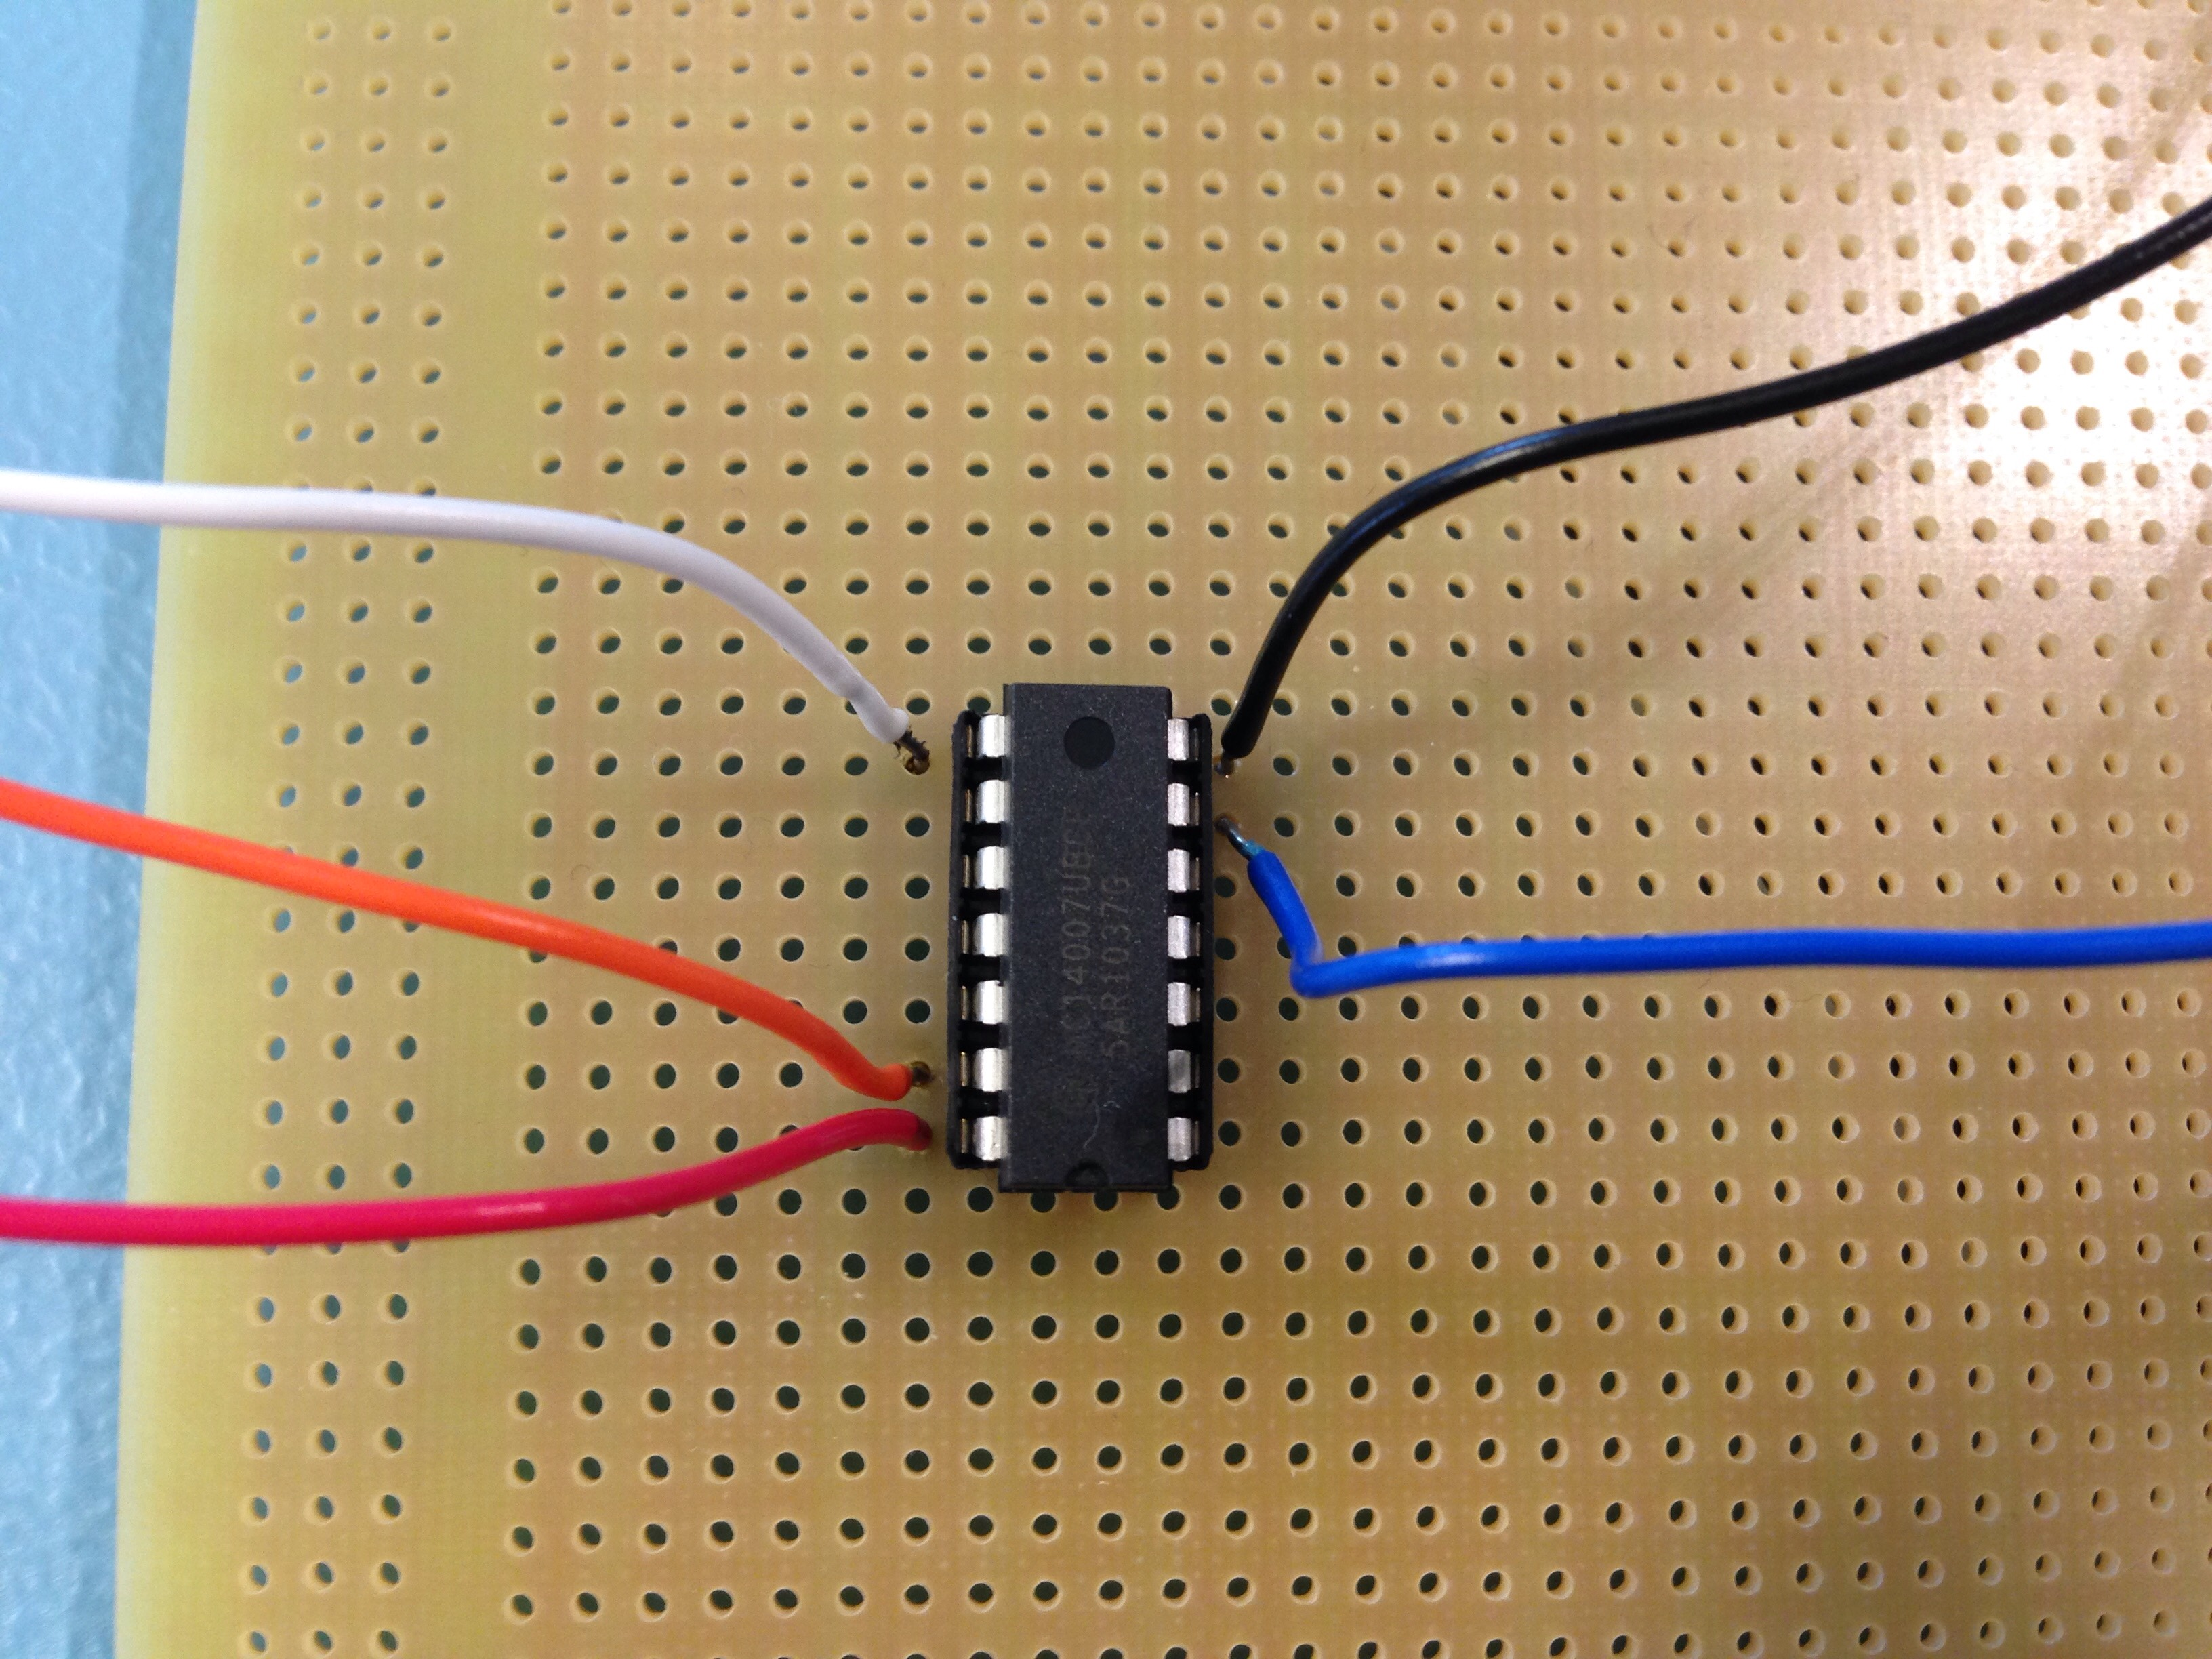
\includegraphics[width=0.5\textwidth]{img/Transistor_setup.jpg}}
  \caption{Transistor setup.}
  \label{fig:tran-setup}	
\end{figure}
\newpage
\begin{figure}[!htbp]
 \centering
  \fbox{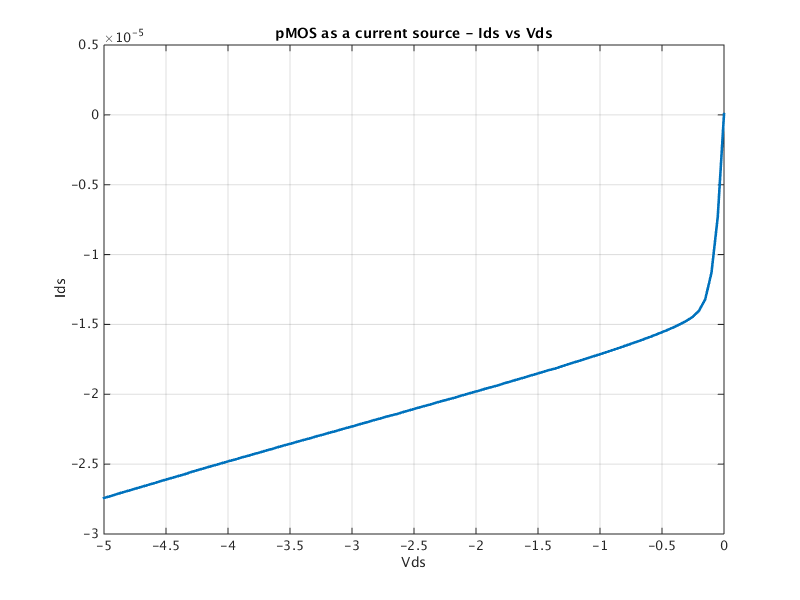
\includegraphics[width=\textwidth]{img/task1_pmos_as_a_current_source.png}}
  \caption{pmos as a current source.}
  \label{fig:pmos-as-current-source}	
\end{figure}    
\newpage
%//////////////////////////////////////Task2///////////////////////////////////////////////////////////////////////
\section{Task 2}
Now we extend our circut to a current source with a cascode transistor. This transistor also need proper biasing. 
The bias for the new transistor is also set by potentiometer as seen i figure \ref{fig:sch:task2}.\\
\begin{figure}[htbp]
 \centering
  \fbox{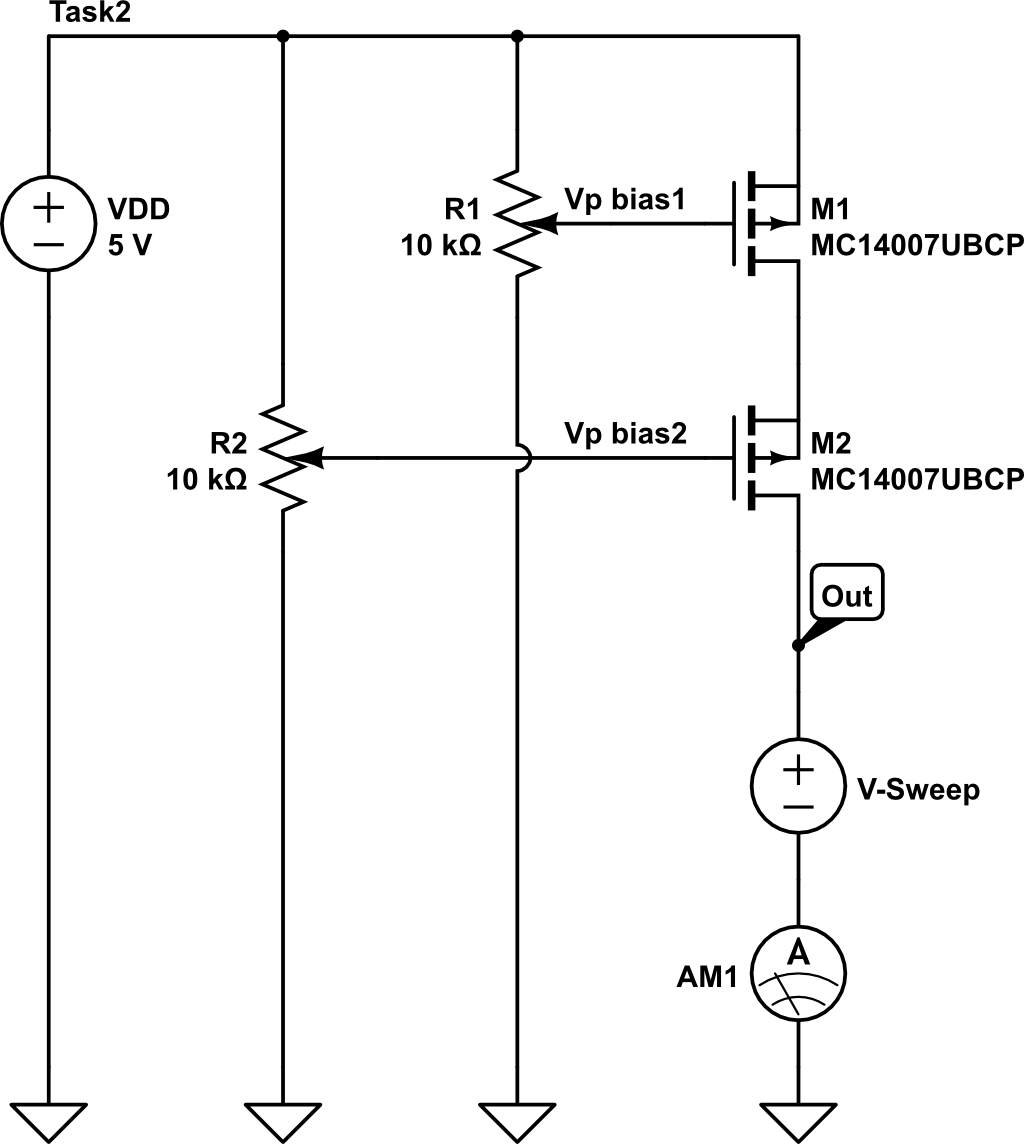
\includegraphics[width=0.5\textwidth]{img/inf4411_lab2_task2_schematics}}
  \caption{Shematic for two pMOS transistors.}
  \label{fig:sch:task2}	
\end{figure}\\
Now the minimal voltage difference between $V_{DD}$ and $V_{p\_bias2}$ is $3.39 V$ relative to $V_{DD}$ in order to get the circuit 
to act as an constant current source. Figure \ref{fig:pfet-cascode-pfet} shows a plot of the output current as a function 
of $V_{out}$. \\
The output resistance of this cuircuit is estmated to $13.35 M\Omega$, and 
the minimial voltage $V_{DD} - V_{out}$ for the cuircuit is $5V - 3V = 2V$. \\
\newpage
Figure \ref{fig:pfet-cascode-pfet} shows plot of output current as function of $V_{out}$.
\begin{figure}[!htbp]
 \centering
  \fbox{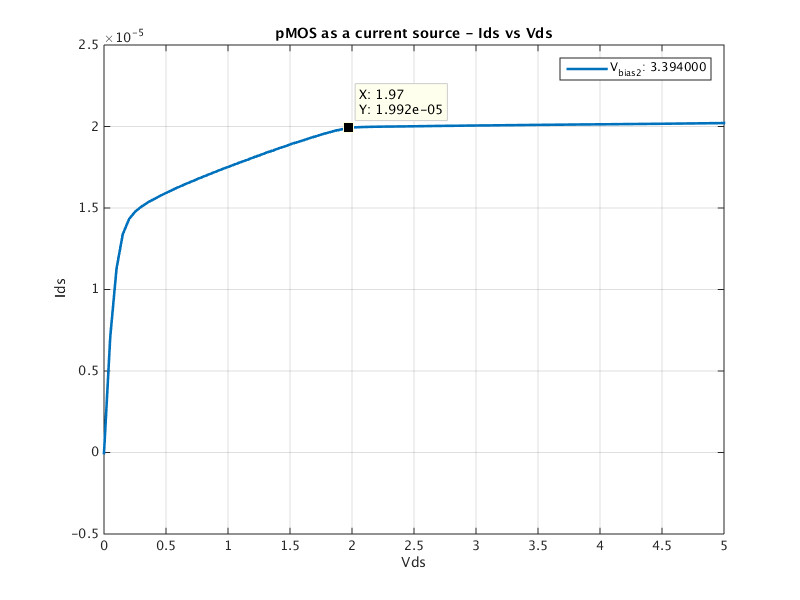
\includegraphics[width=\textwidth]{img/task2_pmos_as_a_current_source.png}}
  \caption{pFET and cascode pFET as a current cource.}
  \label{fig:pfet-cascode-pfet}	
\end{figure}
\newpage
%//////////////////////////////////////Task3///////////////////////////////////////////////////////////////////////
\section{Task 3}
Using the results form task 1 and task 2 we can estimate values for $V_{eff}$ and the treshold voltage $V_{tp}$.
For task 1, $V_{eff}$ is calculated from the relationship $V_{DD} - V_{out}$. For task 2, $V_{eff}$ is calculated from the 
relationship between $V_{out}$ and $V_{p\_bias2}$.\\
\\
In the fisrt task, $V_{eff} = V_{sd} = 0.5V$ and $V_{sg} = V_{p\_bias1} = 1.2V$. This gives $V_{tp} =$ \underline{$-0.7V$}.\\
\\
In the second task, $2V_{eff} = V_{DD} - V_{out} = 2V$ which means $V_{eff} = 1V$  and $V_{sg2} = V_{p\_bias2} = 3.39V$.
This gives  $V_{tp} =$ \underline{$-1.39V$}.
\\
The two estimates are not consistent.

\newpage
%//////////////////////////////////////Task4///////////////////////////////////////////////////////////////////////
\section{Task 4}
In this task we were supose to use two nMOS transistors and repeat what we did in task 2. Figure \ref{fig:sch:task4} shows 
the shematics for this setup. Since the package that was used for the previous task only can be configured for three 
different gate voltages, we had to add an extra package.\\
\\
\begin{figure}[htbp]
 \centering
  \fbox{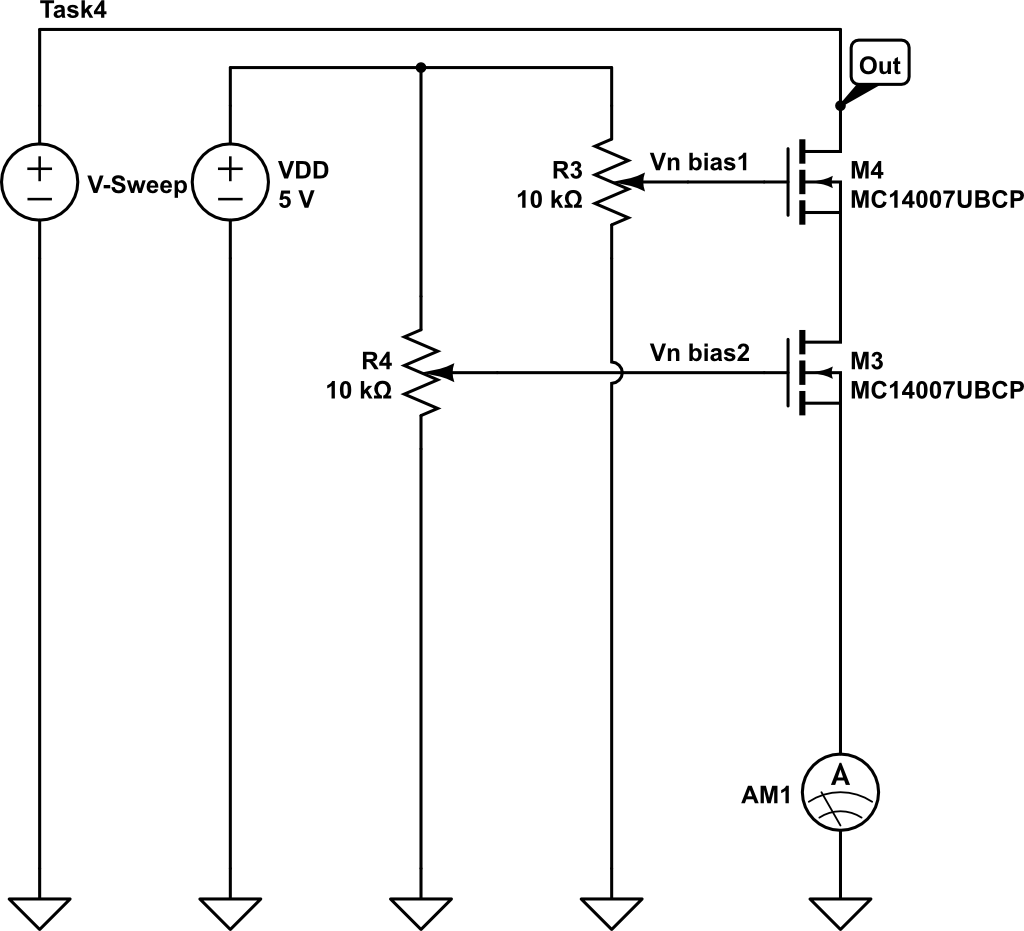
\includegraphics[width=0.5\textwidth]{img/inf4411_lab2_task4_schematics_corrected}}
  \caption{Shematic for two nMOS transistor.}
  \label{fig:sch:task4}	
\end{figure}
\begin{figure}[htbp]
 \centering
  \fbox{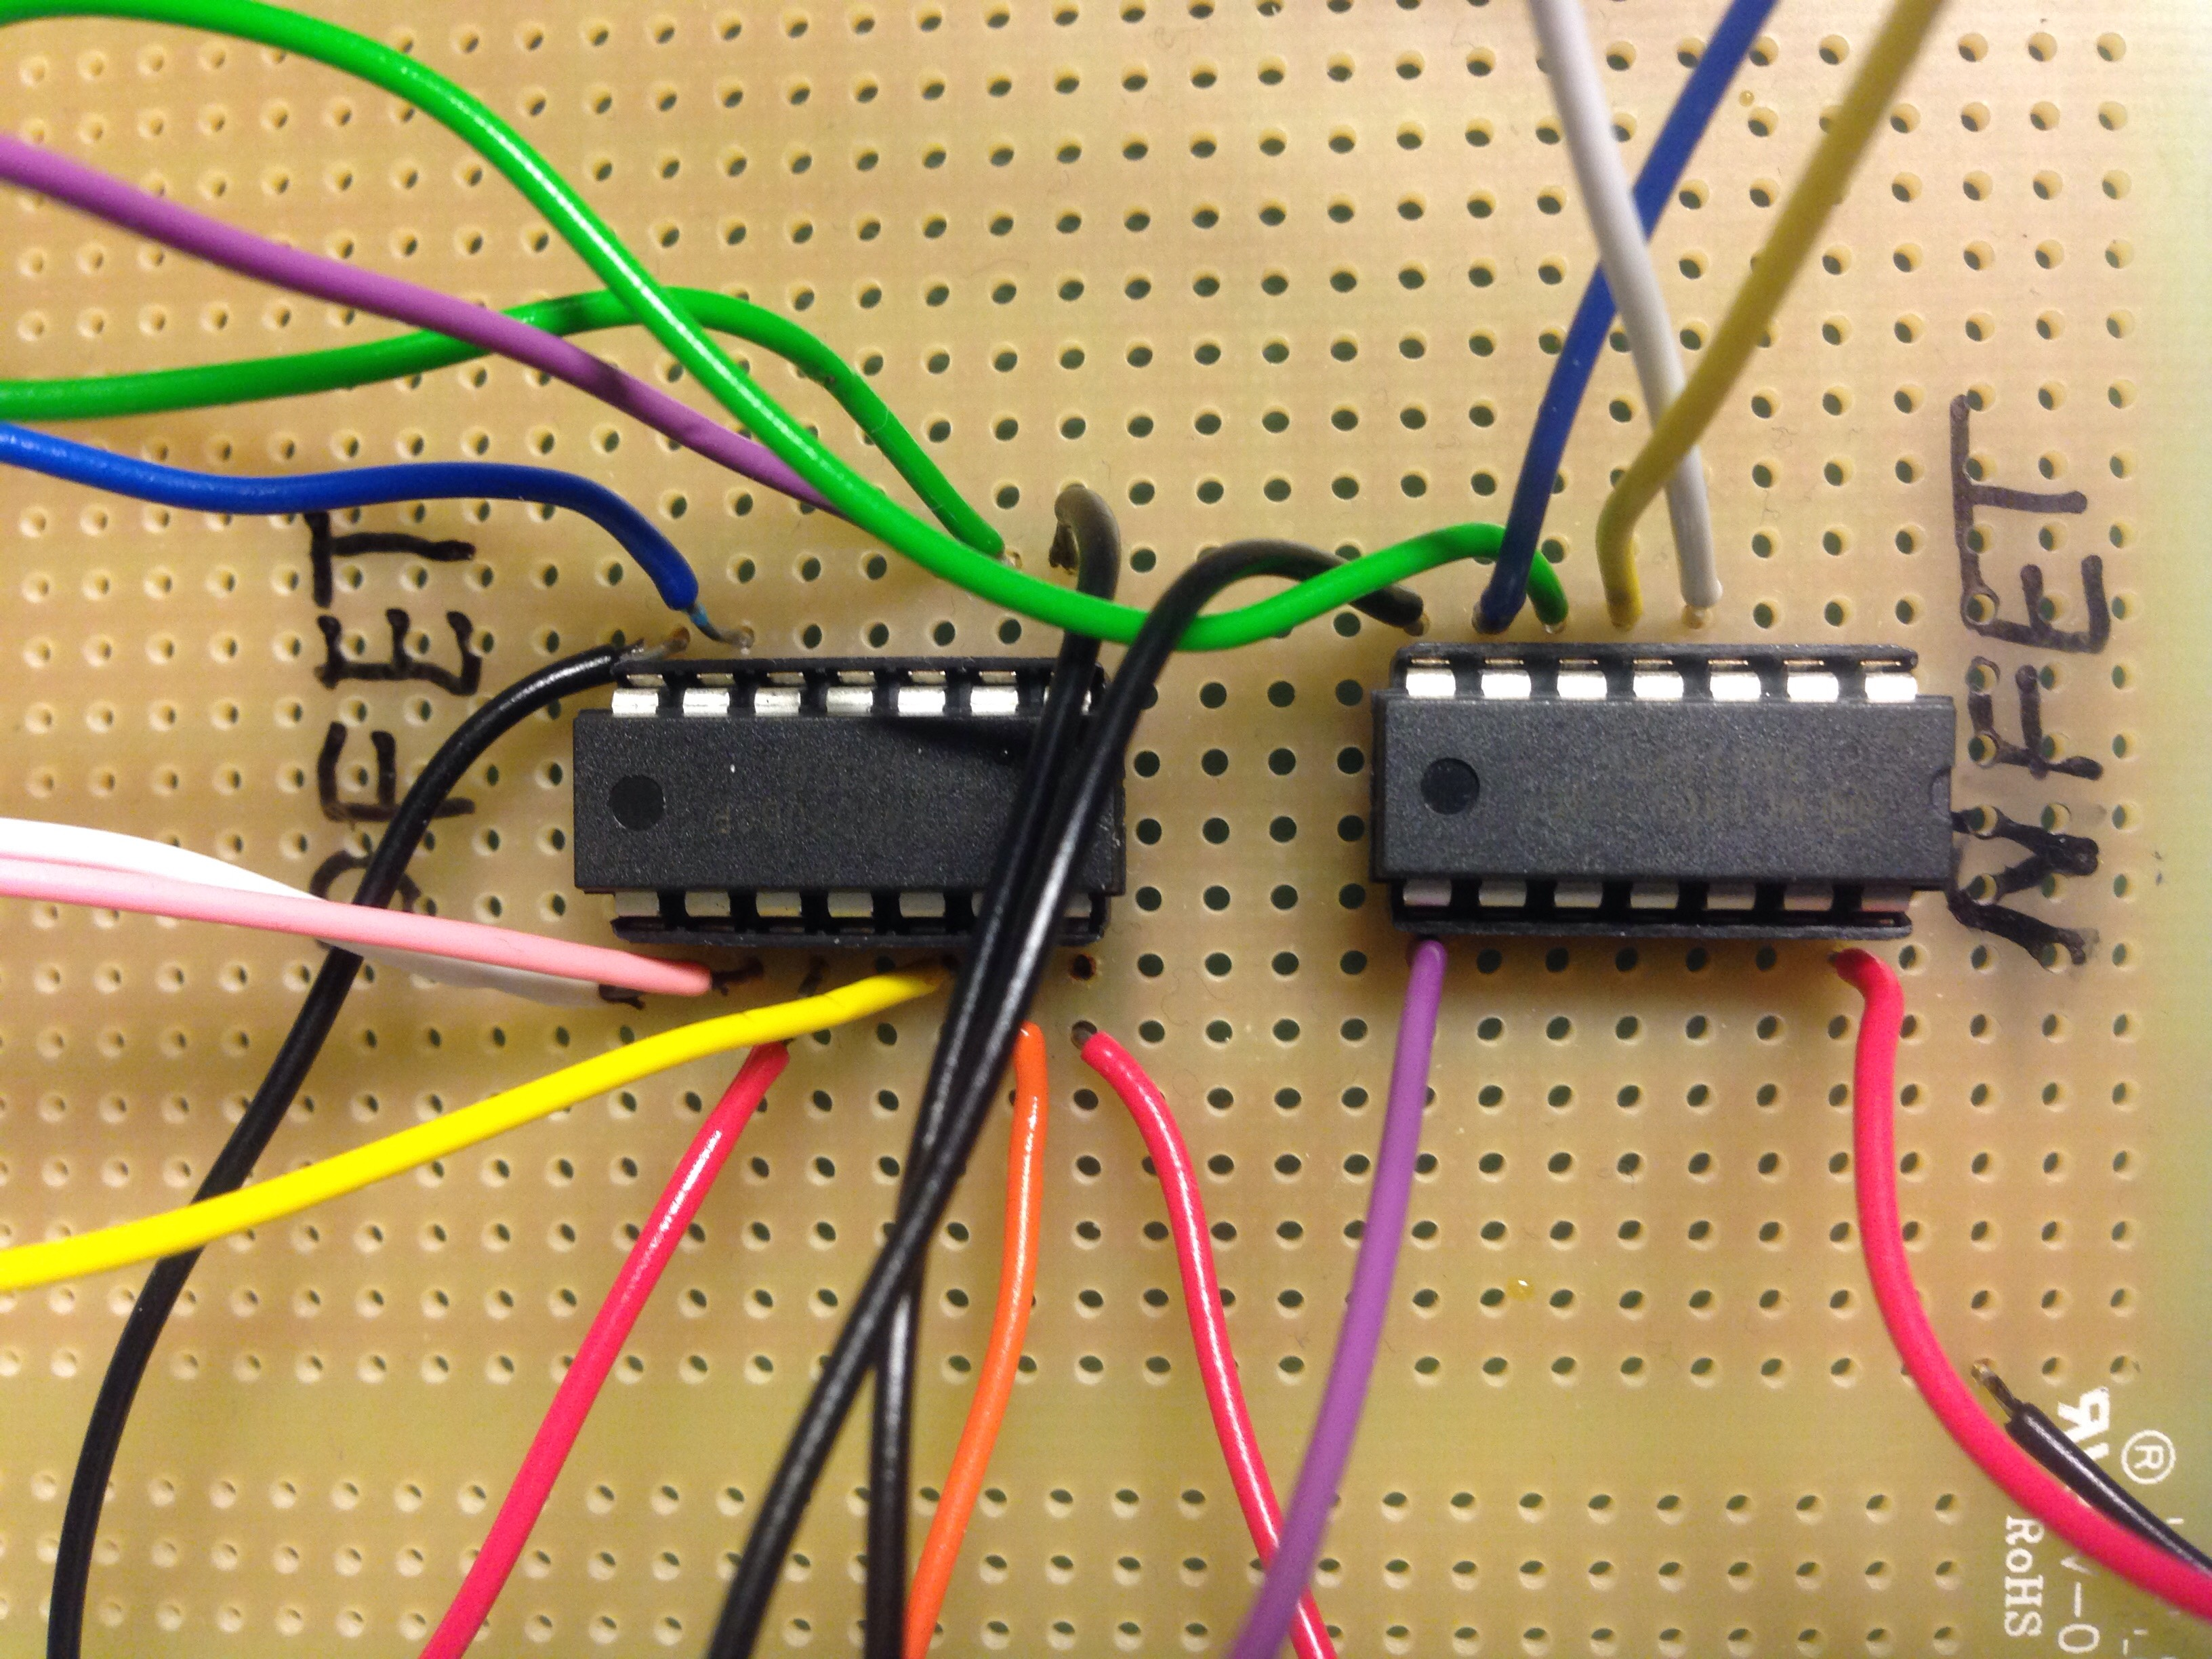
\includegraphics[width=0.6\textwidth]{img/pmos_and_nmos_setup}}
  \caption{pMOS and nMOS PCB setup.}
  \label{fig:pmos_nmos}	
\end{figure}
\\
Also here, we used two potentiometers at $10k\Omega$ to adjust the bias voltages for the nMOS transistors. By using a 
supply voltage at $V_{DD} = 5V$, we adjusted the potentiometers so that the transistors macthed the requirements for a current 
of $20 {\mu}A$. We found the first gate voltage ($V_{in}$) i.e. point of operation of transistor M3 to be $3.39 V$ refered 
to $V_{DD}$.\\ 
\\
This voltage was found by applying $5 V$ at $V_{DD}$ and then keep the sweeping voltage ($V_{sweep}$) constant at $2.5 V$. 
$V_{sweep}$ is kept constant in order to get a wide range above and below $I_D$ of $20 {\mu}A$.\\
\\
The second gate voltage ($V_{n\_bias}$) for transistor M4, was then selected by keeping $V_{DD}$, $V_{n\_bias}$ and $V_{in}$ 
constant at the respectively voltages $5$, $2.5$ and $3 V$.Then the potensiometer was adjusted to mach the requrement for $20 {\mu}A$. 
This voltage was found to be $1.95 V$ refered to $V_{DD}$.\\
\\
$V_{n\_bias}$ is set somewhat bigger than minimum value in order to keep both nMOS transistors in deep saturation and in order to
keep the point of operation in linear region.\\
\\
By finding $r_{out}$ we divided the delta voltage by the delta current (${\Delta V}/{\Delta I} = r_{out}$) and got \underline{$28M {\Omega}$}.\\
\\
The plot of the current as a function of the voltage is shown in Figure \ref{fig:task4_plot}.\\ 

\begin{figure}[htbp]
 \centering
  \fbox{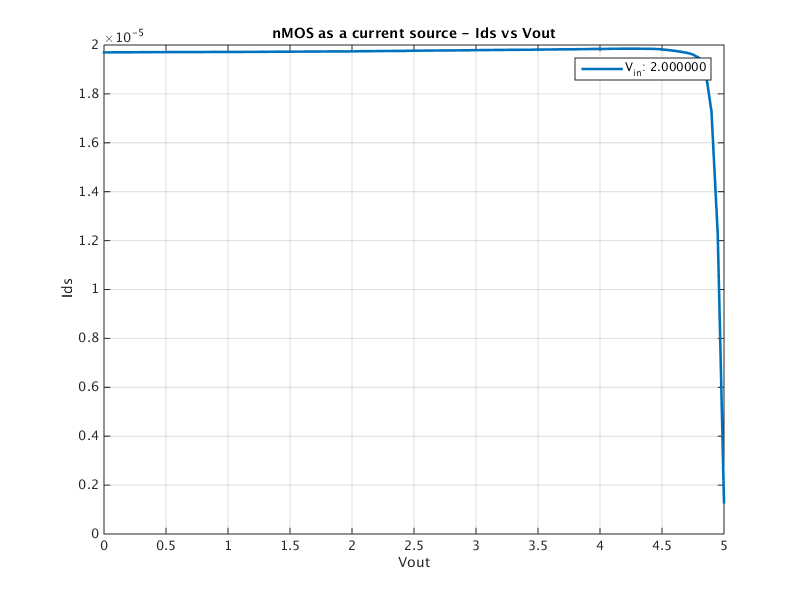
\includegraphics[width=\textwidth]{img/task4_nmos_as_a_current_source}}
  \caption{nMOS transistor as current source.}
  \label{fig:task4_plot}	
\end{figure}
\newpage
%//////////////////////////////////////Task5///////////////////////////////////////////////////////////////////////
\section{Task 5}
We now want to determine a good DC voltage for the input for the amplifier. Since our goal is to have an output voltage 
verry close to $Vdd/2$, we need to find good bias voltages for $V_{n\_bias1}$ and $V_{in}$. We found this volage to be $16 V$, 
in order to ensure that all transistors are operating. For the bias voltages we used the same relationships to $Vdd$ as in the previos tasks.\\
\\
Tabel:\\
\begin{enumerate}
\item \itab{$V_{DD}$:} \tab{16 V}
\item \itab{$V_{p\_bias1}$:} \tab{1.196 V}
\item \itab{$V_{p\_bias2}$:} \tab{3.39 V}     
\item \itab{$V_{n\_bias}$:} \tab{3.01 V}  
\item \itab{$V_{sweep}$} \tab{0 - 6 V}
\end{enumerate}
Note: All voltages is with respect to $V_{DD}$.\\ 
\\
The plot of the measurement is shown in Figure \ref{fig:lin-amp}.\\
\\
\begin{figure}[htbp]
 \centering
  \fbox{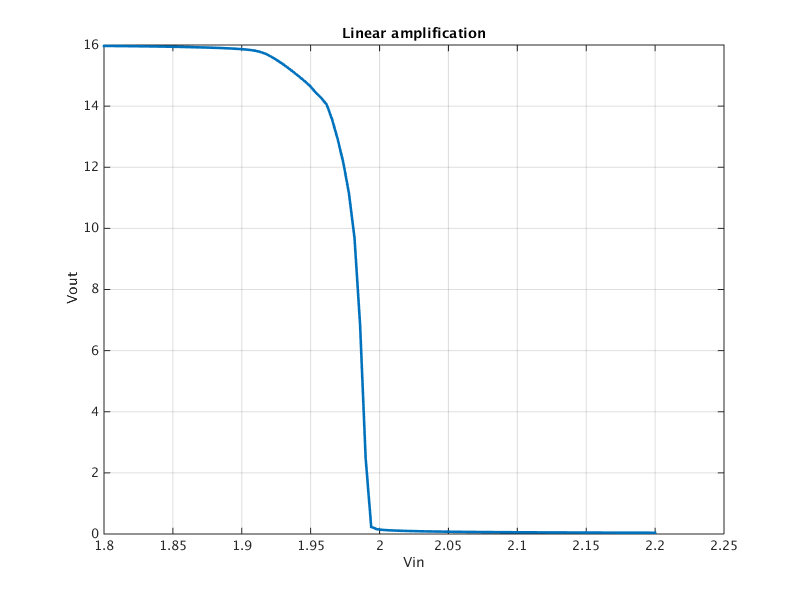
\includegraphics[width=\textwidth]{img/task5_vin_vs_vout}}
  \caption{Linear amplification.}
  \label{fig:lin-amp}	
\end{figure}
\\
The input range for which the amplifier behaves linearly is approximantely between $1.962 V$ and $1.994 V$ which is $32mV$. 
The output linear range is between $14.05 V$ and $0.2334 V$ which is $13.82 V$.\\
\\
From the plot in Figure \ref{fig:lin-amp-tan}, we find the the amplification to be $A_v = -619.25$.\\
The center of the linear region is in the point $(1.9847 , 7.7073)$ in the plot in Figure \ref{fig:lin-amp-tan}.\\
Equation for linear approximation is $V_{out} = A_v ( V_{in} - 1.9847 ) + 7.7073$. The linear approximation plot is 
shown in Figure \ref{fig:lin-amp-tan}.\\
\begin{figure}[htbp]
 \centering
  \fbox{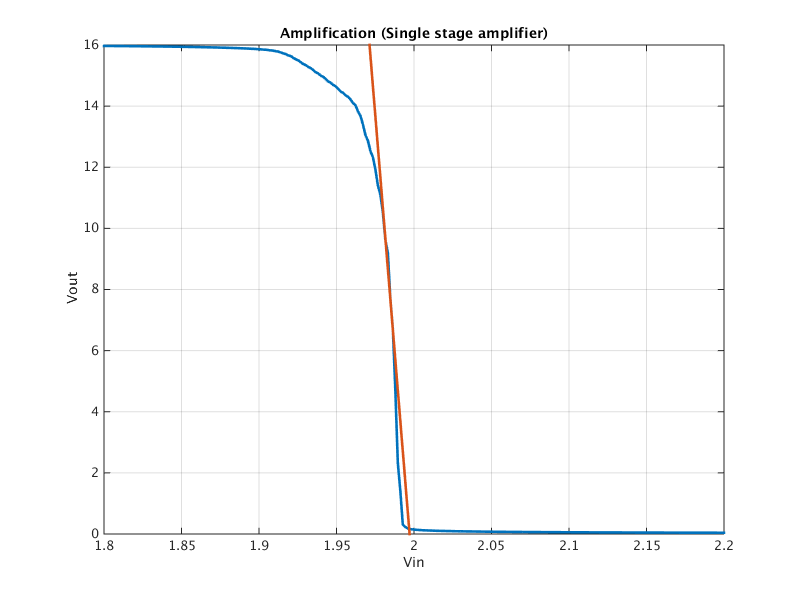
\includegraphics[width=\textwidth]{img/task5_single_stage_amplifier_tangent}}
  \caption{Linear amplification with tangent line.}
  \label{fig:lin-amp-tan}	
\end{figure}
\newpage
%//////////////////////////////////////Task4///////////////////////////////////////////////////////////////////////
\section{Task 6}
Our configuration of cascoded amplifier is a telescopic cascade amplifier whose voltage gain is given as
$Av = -g_m || R_L$
where $g_m$ is product of transconductance of M3 and M4 and $R_L$ is result of parallel resitance from task 2 and task 4.\\
\\
A plot of $I_{DS}$ and $V_{in}$ is shown in Figure \ref{fig:ids_vs_vin}.\\
\begin{figure}[htbp]
 \centering
  \fbox{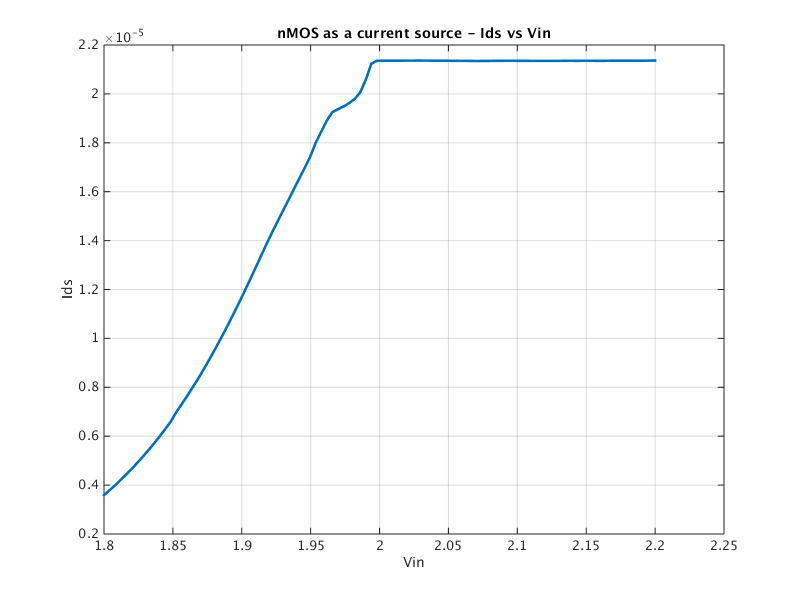
\includegraphics[width=\textwidth]{img/task5_vin_vs_ids}}
  \caption{$I_{DS}$ as funtion of $V_{in}$.}
  \label{fig:ids_vs_vin}	
\end{figure}
\newpage
%//////////////////////////////////////Task4///////////////////////////////////////////////////////////////////////
\section{Task 7}
We were not able to comlete this task. It was very difficult to make a proper value for the AC signal to be mesured.\\
We did also have some problems connecting the oscillosope together with Matlab.

\section{Picture of the final PCB}
Picture of the final PCB board.\\
\begin{figure}[htbp]
 \centering
  \fbox{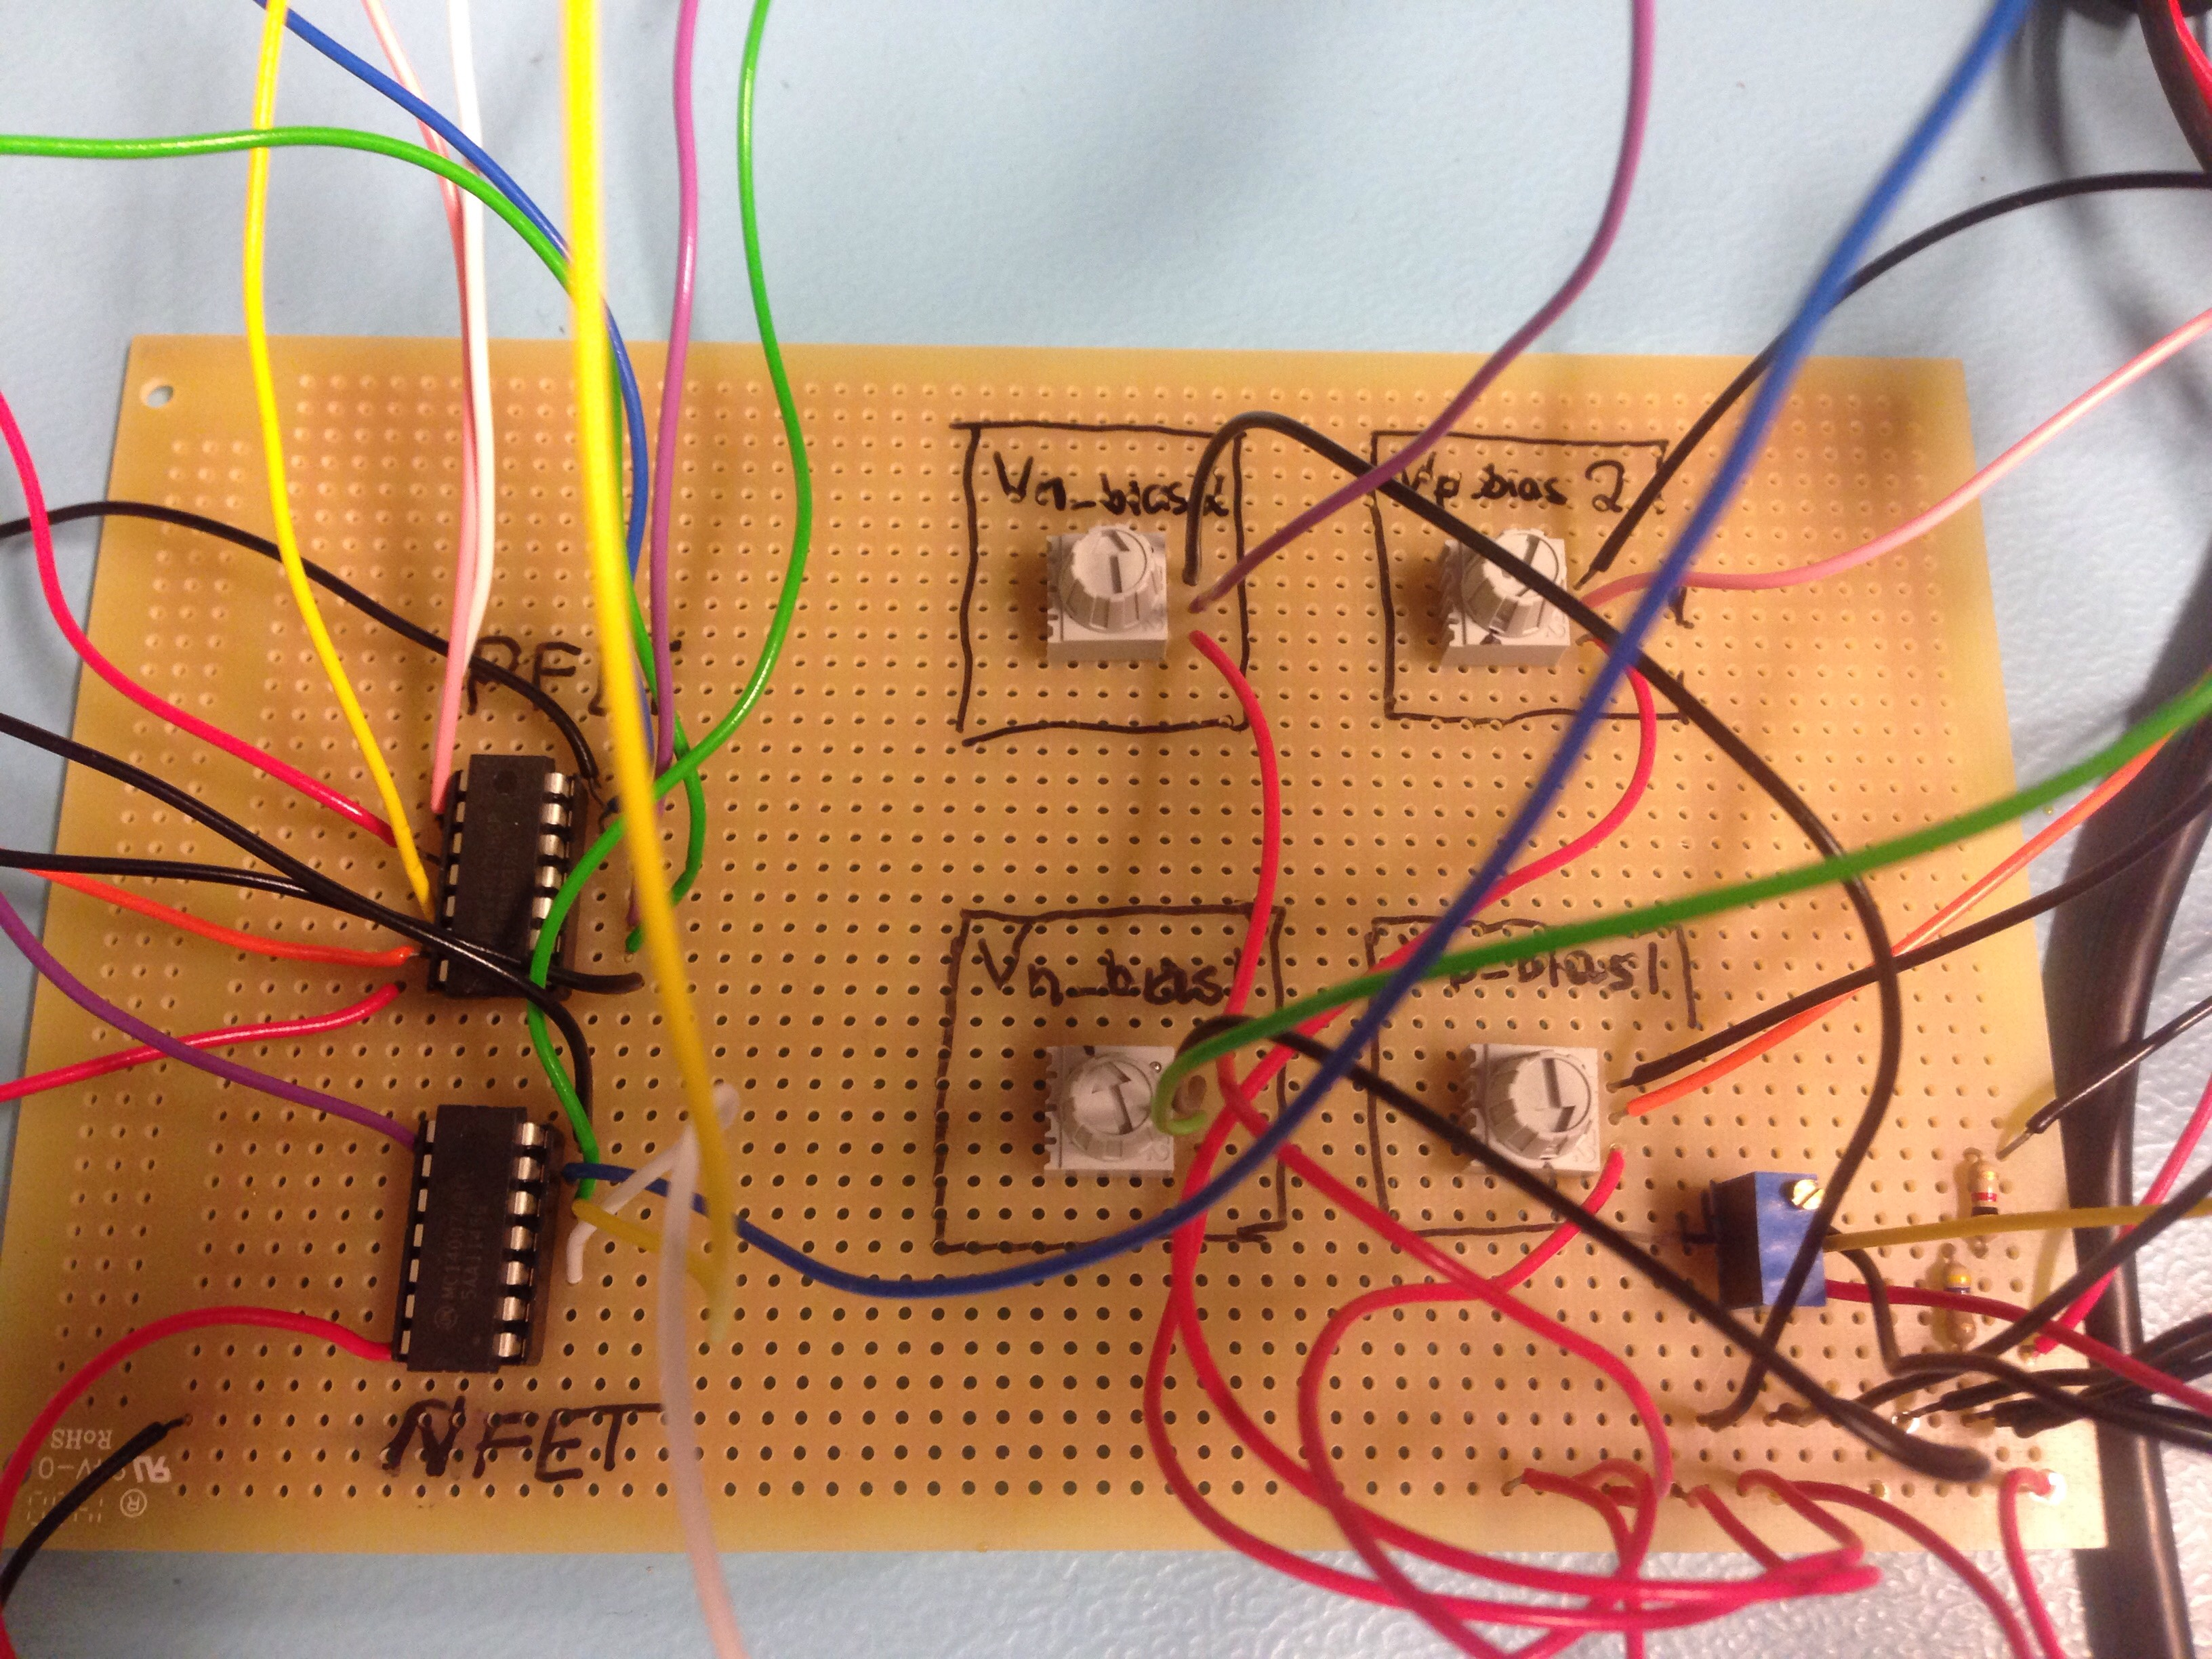
\includegraphics[width=\textwidth]{img/pcb_setup}}
  \caption{Final PCB board.}
  \label{fig:pcb}	
\end{figure}



\end{document}
